\documentclass[twocolumn]{article}
\usepackage[english]{babel}
\usepackage[utf8]{inputenc}
\usepackage{amsmath,amssymb,physics,mathtools,blindtext,graphicx,float}
\usepackage[a4paper,total={7.5in,10in}]{geometry}
\usepackage[labelfont=bf]{caption}

\begin{document}
\begin{large}
\section*{Assignment 6: Explaining the periodic table}
\subsection*{Introduction}
In this report, an attempt is made to qualitatively understand general atomic systems by using a mean field approximation. The charge density resulting from the occupied orbitals of an atomic system can be written as 
\begin{equation}
    \rho(r,\theta,\varphi) = \sum_{n=1}^{N}\sum_{\ell=0}^{n-1}\sum_{m=-\ell}^{\ell}g_{n\ell m}\rho_{n\ell m}(r,\theta,\varphi)
\end{equation}
where $g_{n\ell m}$ takes the value zero, one or two which is the number of electrons occupying the $(n,\ell,m)$ state, and $\rho_{n\ell m}$ is the charge density of an electron in the $(n,\ell,m)$ state:
\begin{equation}
    \begin{split}
        \rho_{n\ell m}(r,\theta,\varphi) &= -e\left|\psi_{n\ell m}(r,\theta,\varphi)\right|^2 \\ 
        &= -eR^2_{n\ell}(r)\left|Y_{\ell m}(\theta,\varphi)\right|^2
    \end{split}
\end{equation}
where $R$ is the radial wave function and $Y$ are the spherical harmonics. We'll replace the spherical harmonic with its average
\begin{equation}
    \begin{split}
        &\left|Y_{\ell m}(\theta,\varphi)\right|^2 \\ 
        &\hspace{0.3cm}\to \frac{1}{4\pi}\int\limits_{\theta=0}^\pi\int\limits_{\varphi=0}^{2\pi}\left|Y_{\ell m}(\theta,\varphi)\right|^2r^2\sin\theta\text{d}\theta\text{d}\varphi = \frac{1}{4\pi}
    \end{split}
\end{equation}
so that $\rho_{n\ell m} \to -eR^2_{n\ell}/4\pi$. This enables us to write 
%We notice that different $m$ give the same charge distribution for fixed $n$ and $\ell$, i.e. $\rho_{n\ell m} = \rho_{n\ell m'}$. This enThus, we define $g_{n\ell}$ to be the number electrons being in a state with principal and azimuthal quantum number $(n,\ell)$ so that we can write 
\begin{equation}
    \label{30apr1108}
    \rho(r) = -\frac{e}{4\pi}\sum_{n=1}^{N}\sum_{\ell=0}^{n-1}g_{n\ell}R^2_{n\ell}(r)
\end{equation}
where $g_{n\ell}$ is the number electrons being in a state with principal and azimuthal quantum number $(n,\ell)$ and $\rho(r)$ is to be understood as the approximation of $\rho(r,\theta,\varphi)$ in which we have averaged over the spherical harmonics.

The radial wavefunctions are solutions to 
\begin{equation}
    \label{30apr1107}
    \begin{split}
        &E_{n\ell}(rR_{n\ell}) = -\frac{\hbar^2}{2m}\frac{\text{d}^2\left(rR_{n\ell}\right)}{\text{d}r^2}  \\ 
        &\hspace{0.3cm} + \left[\frac{\hbar^2\ell(\ell+1)}{2mr^2}-\frac{Ze^2}{4\pi\epsilon_0r}-e\varphi_{ee}(r)\right](rR_{n\ell}) 
    \end{split}
\end{equation}
where $P_{n\ell} = rR_{n\ell}$ is the reduced radial wavefunction and $\varphi_{ee}(r)$ is a yet unknown electric potential. It is decomposed into two parts 
\begin{equation}
    \varphi_{ee} = \varphi_{ee}^{dir} + \varphi_{ee}^{exch}
\end{equation}
where the direct part is the solution to the Poisson equation
\begin{equation}
    \label{30apr1122}
    \frac{\text{d}^2(r\varphi_{ee}^{dir}(r))}{\text{d}r^2} +\frac{r\rho(r)}{\epsilon_0} = 0
\end{equation} 
with boundary conditions that $r\varphi_{ee}^{dir}$ should vanish at the origin and that $r\varphi_{ee}^{dir}$ should approach $-Ze/4\pi\epsilon_0$ as $r\to\infty$. The exchange part is calculated with the formula
\begin{equation}
    \label{30apr1123}
    \varphi_{ee}^{exch}(r) = \frac{3e}{4\pi\epsilon_0}\left|\frac{3\rho(r)}{8\pi e}\right|^{1/3}.
\end{equation}
To determine the right $\varphi_{ee}^{dir}$, the system was solved iteratively until it became self-consistent. 

\subsection*{Numerical implementation}
The implementation can be summarized with the following steps:
\begin{itemize}
    \item[1.] Set $\varphi_{ee}=0$.
    \item[2.] Calculate $\rho(r)$ by solving \eqref{30apr1107} for the different $n$ and $\ell$ and calculating the sum in \eqref{30apr1108}.
    \item[3.] Use $\rho(r)$ to solve Poisson's equation \eqref{30apr1122} and obtain from it the potential $\varphi_{ee}^{dir}$.
    \item[4.] Calculate the exchange potential $\varphi_{ee}^{exch}$ using equation \eqref{30apr1123} and set $\varphi_{ee} = \varphi_{ee}^{dir} + \varphi_{ee}^{exch}$. 
    \item[5.] Repeat from 2. until convergence of energies $E_{n\ell}$. 
\end{itemize}
Atomic units were used (for more details, see end of report).

\subsection*{Test on helium atom}
For helium, the charge distribution takes the simple form
\begin{equation}
    \rho(r) = -\frac{e}{4\pi}\cdot 2R^2_{10}(r).
\end{equation}
Applying the steps above, the energy converges to the value $E_{10} = -0.76$ Hartree (see figure \ref{5maj0820}). The electric potential $\varphi_{ee}$ after six iterations is plotted in figure \ref{5maj0822}.
\begin{figure}[t]
    \includegraphics[scale=0.35]{Heliumenergy.png}
    \caption{The energy $E_{10}$ as a function of iteration step for the helium atom. The energy converges to a value $E_{10}=-0.76$ Hartree.}
    \label{5maj0820}
\end{figure}
\begin{figure}[h]
    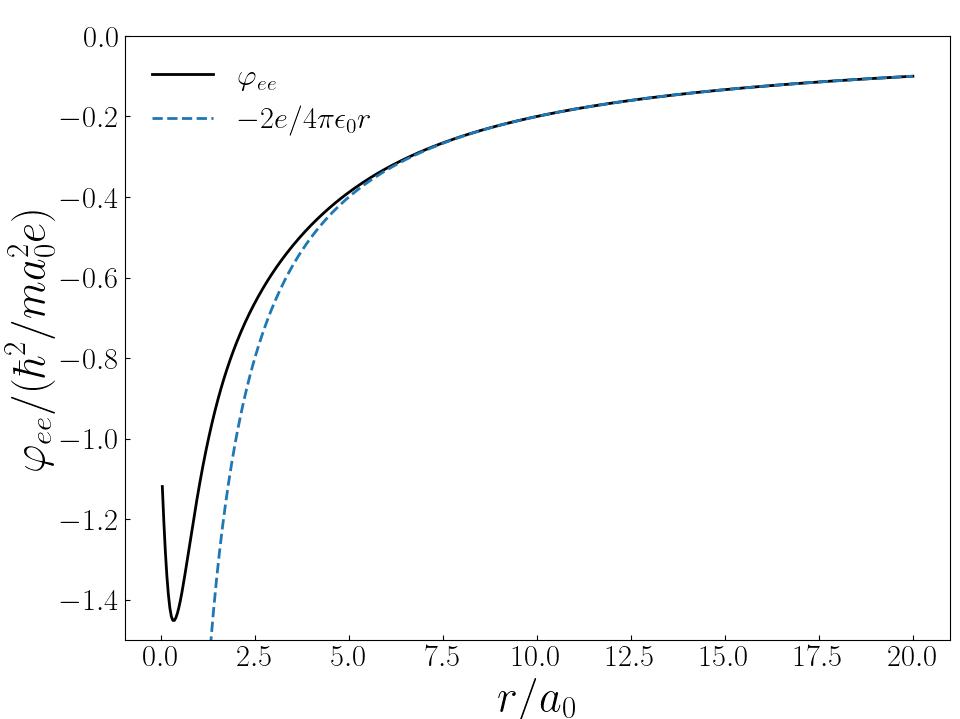
\includegraphics[scale=0.35]{HeliumPhiee.png}
    \caption{The electric potential $\varphi_{ee}$ for the helium atom after six iterations. The potential should converge to the Coulomb potential for large $r$.}
    \label{5maj0822}
\end{figure}
To calculate the total energy, the following formula was used:
\begin{equation}
    E_{tot} = -2E_{10} - \frac{1}{2}\int\limits_0^{r_{max}}P_{10}^2(r)e\varphi_{ee}\text{d}r
\end{equation}
The integral above was calculated numerically and found to be equal to $-0.92$ which gies a total energy of $E_{tot}=-1.06$. 

\subsection*{Other atoms}
The method seemed to work fine for the Helium atom but I didn't get it to work for Neon. The problem was that when I was solving for $rR_{n\ell}$ with a non-zero $\varphi_{ee}$, I got unbound solutions in the iteration, like this one:
\begin{center}
    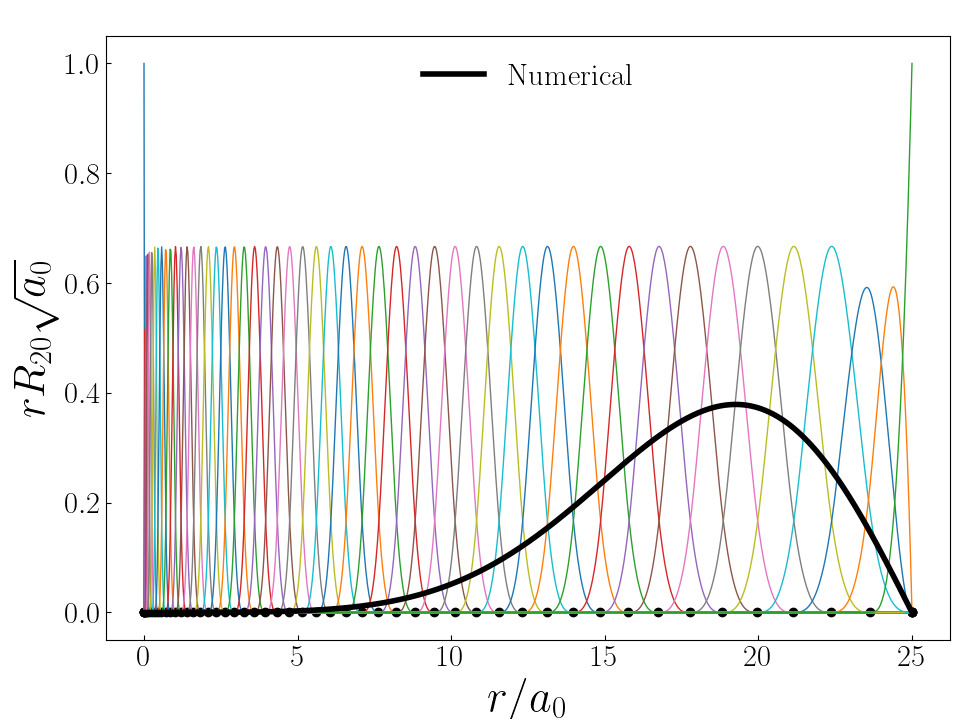
\includegraphics[scale=0.35]{neon.png}
\end{center}
I haven't been able to locate the problem yet, but it could be a sign error somewhere or that I'm implementing the Poisson equation incorrectly.


\subsection*{Units}
%With $V_{ee}=0$, we get a numerical solution on $(0,1)$, $u(\xi)$, where $\xi = r/a_0D$. Then,
%\begin{equation}
%    rR_{n\ell}(r) = \frac{u_{n\ell}(r/a_0D)}{\sqrt{a_0D}}
%\end{equation}
%The distribution is then 
%\begin{equation}
%    \rho(r) = -e\sum_{n,\ell}g_{n\ell}R_{n\ell}^2.
%\end{equation}
%Insert this into 
%\begin{equation}
%    \begin{split}
%        0 &= \frac{\text{d}(rV_{ee}^{dir})}{\text{d}r^2} + r\rho(r)/\epsilon_0  \\ 
%        &= \frac{1}{(a_0D)^2}\frac{\text{d}^2(\alpha\lambda)}{\text{d}\xi^2} - \frac{e}{\epsilon_0}\sum_{n,\ell}g_{n\ell}\frac{u_{n\ell}^2(\xi)}{(a_0D)^2\xi}
%    \end{split}
%\end{equation}
%so set $\alpha=-e/\epsilon_0$ such that
%\begin{equation}
%    \frac{\text{d}^2\lambda}{\text{d}\xi^2} + \sum_{n,\ell}g_{n\ell}\frac{u_{n\ell}^2(\xi)}{\xi} = 0
%\end{equation}
%Which becomes 
%\begin{equation}
%    \lambda'' + \xi\sigma(\xi) = 0
%\end{equation}
%where 
%\begin{equation}
%    \sigma(\xi) = \sum_{n,\ell} g_{n\ell}\frac{u^2_{n\ell}}{\xi^2}
%\end{equation}
%The boundary conditions are $\lambda(0) = 0$ and $\lambda(1) = N/4\pi$ (check). From this we have
%\begin{equation}
%    rV_{ee}^{dir} = \alpha\lambda(r/a_0D)
%\end{equation}
%or 
%\begin{equation}
%    V_{ee}(r) = -\frac{e}{\epsilon_0r}\lambda(r/a_0D)
%\end{equation}
%which should be negative.
%
%The new radial wavefunction is then given by
%\begin{equation}
%    \begin{split}
%        &-\beta^2\left[u'' - \frac{\ell(\ell+1)}{\xi^2}u + \frac{2}{\beta}\left(\frac{1}{\xi}-\frac{4\pi\lambda(\xi)}{Z\xi}\right)u\right] \\ 
%        &\hspace{1cm}= E'u
%    \end{split}
%\end{equation}

Defining $u_{n\ell}$ to be the numerical solution to $rR_{n\ell}$ and making the substitutions
\begin{equation}
    \xi = r/a_0,\quad E' = E/(\hbar^2/a_0^2m),\quad u = a_0^{1/2}rR_{n\ell},
\end{equation}
the radial function becomes
\begin{equation}
    \label{5maj1822}
    -\frac{1}{2}u'' + \left[\frac{\ell(\ell+1)}{2\xi^2}-\frac{mea_0^2}{\hbar^2}(\varphi_C+\varphi_{ee})\right]u = E'u.
\end{equation}
The direct part of $\varphi_{ee}$ is the solution to the Poisson equation:
\begin{equation}
    (r\varphi_{ee}^{dir})'' + r\rho(r)/\epsilon_0 = 0.
\end{equation}
Now, define 
\begin{equation}
    \hat{\varphi}_{ee}^{dir} = \frac{\varphi_{ee}^{dir}}{\hbar^2/(ma_0^2e)}
\end{equation}
and set $\sigma = \rho/B$ where $B$ is to be determined. Making these substituions, and setting $r=a_0\xi$, we get
\begin{equation}
    \label{5maj1821}
    (\xi\hat{\varphi}_{ee}^{dir})'' + \frac{4\pi a_0^3}{e}B\sigma(\xi)\xi = 0.
\end{equation}
So if we let $B=e/(4\pi a_0^3)$, we get 
\begin{equation}
    (\xi\hat{\varphi}_{ee}^{dir})'' + \xi\sigma(\xi) = 0.
\end{equation}
The Coulomb part is always the same,
\begin{equation}
    \hat{\varphi}_C = \frac{\varphi_C}{\hbar^2/(ma_0^2e)} = \frac{Z}{\xi}.
\end{equation}




\end{large}
\end{document}
